\documentclass[11pt,a4paper]{article}
\usepackage[utf8]{inputenc}
\usepackage[dutch]{babel}
\usepackage{pgfplots}
\usepgfplotslibrary{units}
\usepackage{float}
\usepackage{amsmath,amsthm}
\usepackage{amsfonts}
\usepackage{amssymb}
\usepackage[left=2cm,right=2cm,top=2.5cm,bottom=2cm]{geometry}
\usepackage{graphicx}
\usepackage{multicol}
\usepackage{enumerate}
\usepackage{fancyhdr}
\pagestyle{fancy}
\usepackage{algorithm}
\usepackage{algpseudocode}
\usepackage{pgfplots}
\usepackage{multirow}
\usepackage{tikz}
\usetikzlibrary{calc}

\floatname{algorithm}{Algoritme}


\usepackage[font=small,labelfont=bf]{caption}
\captionsetup[table]{aboveskip=-0.8em}
\captionsetup[table]{belowskip=-0.7pt}


\lhead {DAIII Project: punten plaatsen} 
\chead{BAZ(~ \thepage ~ )NGA} 
\rhead{Robbert Gurdeep Singh}


\cfoot{} % get rid of the page number 

\usepackage{hyperref}
\usepackage{chngcntr}
\counterwithin*{section}{part}
\counterwithin{algorithm}{section}
\counterwithin{table}{section}
\counterwithin{figure}{section}

\hypersetup{
    colorlinks=false,
    pdfborder={0 0 0},
}

\author{Robbert Gurdeep Singh}
\title{{Project Algoritmen en datastructuren III}\\ \Huge Genetische algoritmen}
%\date{}



\pgfplotsset{compat=1.8}


\newcommand{\drawGraph}[4]{
\begin{tikzpicture}
\begin{axis}[scale only axis, 
	%x-as	
    xmin=0,
	xlabel=#1,	
	%y-as
	ylabel=#2,
	ymin=0,
	%Style
	height=5em,width=.37\textwidth,
	enlargelimits=0.05,
	grid=major,	legend pos=south east
]
#3
\end{axis}
\end{tikzpicture}
}


\newcommand{\lxaxis}[3]{\begin{tikzpicture}
\begin{axis}[scale only axis, 
cycle list name=exotic,
    xmode=log,
    log ticks with fixed point,
	%x-as	
	xlabel=#2,	
	%y-as
	ylabel=#1,
	ymin=0,
	%Style
	height=5em,width=.37\textwidth,
	enlargelimits=0.05,
	grid=major,	legend pos=south east
]
#3

\end{axis}
\end{tikzpicture}}

\newcommand{\rlxaxis}[3]{\begin{tikzpicture}
\begin{axis}[scale only axis, 
cycle list name=exotic,
    xmode=log,
    log ticks with fixed point,
	%x-as	
	xlabel=#2,	
	%y-as
	ylabel=#1,
	%Style
	height=5em,width=.37\textwidth,
	enlargelimits=0.05,
	grid=major,	legend pos=south east
]
#3

\end{axis}
\end{tikzpicture}}

\newcommand{\nxaxis}[3]{\begin{tikzpicture}
\begin{axis}[scale only axis,
cycle list name=exotic, 
	%x-as	
    xmin=0,
	xlabel=#2,	
	%y-as
	ylabel=#1,
	ymin=0,
	%Style
	height=5em,width=.37\textwidth,
	enlargelimits=0.05,
	grid=major,	legend pos=south east
]
#3

\end{axis}
\end{tikzpicture}}


\newcommand{\rnxaxis}[3]{\begin{tikzpicture}
\begin{axis}[scale only axis, 
cycle list name=exotic,
	%x-as	
    xmin=0,
	xlabel=#2,	
	%y-as
	ylabel=#1,
	%Style
	height=5em,width=.37\textwidth,
	enlargelimits=0.05,
	grid=major,	legend pos=south east
]
#3

\end{axis}
\end{tikzpicture}}

\newcommand{\itemMB}[1]{
	\item[$\boldsymbol{#1}$:]
}




\newcommand{\abs}[1]{
	\lvert #1 \rvert
}

\newcommand{\addploti}[1]{\addplot table [y=i, x=testValue, col sep=comma] {../../tests/param_results/#1.log};}
\newcommand{\addplotf}[1]{\addplot table [y=f, x=testValue, col sep=comma] {../../tests/param_results/#1.log};}
\newcommand{\addplott}[1]{\addplot table [y=t, x=testValue, col sep=comma] {../../tests/param_results/#1.log};}

\definecolor{mymark}{HTML}{EBB8B8}

\begin{document}

\twocolumn[\begin{@twocolumnfalse}
    \maketitle
\end{@twocolumnfalse}]
% grep  '^[^%]*\s*\\label' * | sed "s/\s\s*/ /g;s/:/+/;s/\+ /+/;s/^/%/" | column -t -s+
%algoritmen_crossover.tex                      \label{sub:crossover}
%algoritmen_crossover.tex                      \label{alg:crossover-1point}
%algoritmen_crossover.tex                      \label{alg:crossover-random}
%algoritmen_inpoly.tex                         \label{sub:algo-pt-in-poly}
%algoritmen_inpoly.tex                         \label{alg:inPolygon}
%algoritmen_mutation.tex                       \label{sub:Mutation}
%algoritmen_mutation.tex                       \label{ssub:MutationAlgorithm}
%algoritmen_mutation.tex                       \label{alg:Mutation}
%algoritmen_mutation.tex                       \label{ssub:MutationImplementation}
%algoritmen_mutation.tex                       \label{ssub:MutationComplexity}
%algoritmen_stochastic_universal_sampling.tex  \label{sub:SUS}
%algoritmen_stochastic_universal_sampling.tex  \label{fig:SUS}
%algoritmen_stochastic_universal_sampling.tex  \label{alg:SUS}
%algoritmen_stochastic_universal_sampling.tex  \label{ssub:SUSComplexity}
%algoritmen.tex                                \label{sec:algoritmen}
%algoritmen_tournament.tex                     \label{sub:tournament}
%algoritmen_tournament.tex                     \label{alg:tournament}
%algoritmen_tournament.tex                     \label{ssub:notetournament}
%param_opt.tex                                 \label{sub:algLoverSelection}
%param_opt.tex                                 \label{graf:algLoverSelection}
%param_opt.tex                                 \label{graf:numIndividus}
%param_opt.tex                                 \label{graf:numLovers}
%param_opt.tex                                 \label{graf:mutationDeltaFig}
%param_opt.tex                                 \label{graf:mutationDeltaTime}
%param_opt.tex                                 \label{graf:mutation1In}
%param_opt.tex                                 \label{graf:selectionPressure}
%param_opt.tex                                 \label{graf:weightingFactor}
%verslag.tex                                   \label{sec:inleiding}
%verslag.tex                                   \label{sec:explainationcode}
%verslag.tex                                   \label{sub:heap}


\part{Genetisch algoritme}
\section{Inleiding}
\label{sec:inleiding}
Het probleem dat we trachten op te lossen is het volgende: %TODO
Als we het vanaf nu hebben over een veelhoek dan bedoelen we een convexe veelhoek.

\subsection{Gebruikte symbolen}
Tenzij anders vermeld betekenen volgende symbolen het volgende:
\begin{itemize}
\itemMB{n} Het aantal te plaatsen punten
\itemMB{X_i} Het i-de individu 
\itemMB{z} Het aantal zijden van de veelhoek
\itemMB{N_p} Populatiegrootte
\itemMB{N_l} Aantal geliefden
\itemMB{P_M} Selectie druk 
\itemMB{f} De fitheidsfunctie \[f(X_k)= \sum_{P_1 \in X_k}\sum_{P_2 \in X_k} \sqrt{d_2(P_1,P_2)} \]
\end{itemize}

%\subsection{Overzicht}
%\tableofcontents

% subsection  (end)
% section inleiding (end)

\section{Algortitmen}

\subsection{Punt in veelhoek}
\label{sub:algo-pt-in-poly}
Eén van de voorwaarden waaraan een oplossing moet voldoen is dat alle punten \textbf{in} de veelhoek liggen.Het is dus noodzakelijk om een algoritme te hebben dat bepaalt of een punt zich al dan niet in de convexe veelhoek bevind.
\subsubsection{Idee}
Trekken we een lijn vanuit het punt ``naar boven'', dan kunnen we 3 gevallen onderscheiden:
\begin{itemize}
\item We snijden de veelhoek niet ($P_{1}$): \\
		We weten dat we ons niet binnen de veelhoek bevonden.
\item We snijden de veelhoek juist 1 keer ($P_{2}$):\\
		Nu zijn we zeker in de veelhoek. 
\item We snijden de veelhoek juist\footnote{Merk op dat indien we de veelhoek meer dan 2 keer snijden, we kunnen aantonen dat de veelhoek niet convex is.} 2 keer ($P_{3}$):\\
		We liggen onder en dus ook buiten de veelhoek.
\end{itemize}

\begin{center}
\begin{figure}[H]
\centering
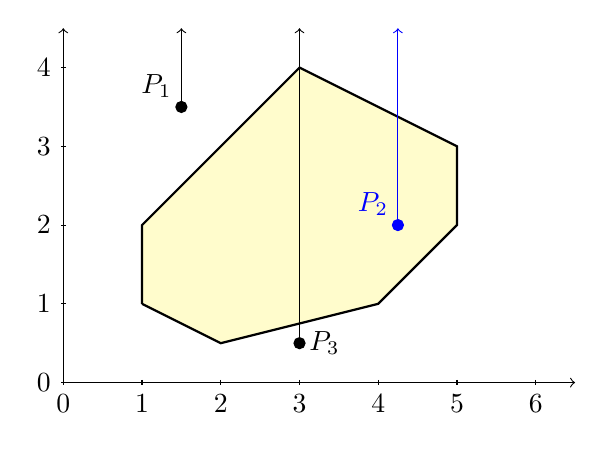
\begin{tikzpicture}
\draw[->] (0,0) -- (6.5,0);
\draw[->] (0,0) -- (0,4.5);

\foreach \x in {0,1,2,3,4,5,6}
    \draw (\x cm,1pt) -- (\x cm,-1pt) node[anchor=north] {\x};
\foreach \y in {0,1,2,3,4}
    \draw (1pt,\y cm) -- (-1pt,\y cm) node[anchor=east] {\y};

\draw[thick,fill=yellow, fill opacity=0.2] 
      (1,1) -- (1,2) -- 
	  (3,4) -- (5,3) -- 
	  (5,2) -- (4,1) -- 
	  (2,0.5) -- (1,1);
	  
	  
\coordinate (out1)    at (1.5,3.5);
\coordinate (out1top) at (1.5,4.5);
\filldraw[black] (out1) circle (2pt) node[anchor=south east] {$P_{1}$};

\coordinate (out2)    at (4.25,2);
\coordinate (out2top) at (4.25,4.5);
\filldraw[blue] (out2) circle (2pt) node[anchor=south east] {$P_{2}$};

\coordinate (out3)    at (3,0.5);
\coordinate (out3top) at (3,4.5);
\filldraw[black] (out3) circle (2pt) node[anchor=west] {$P_{3}$};


\draw[->] (out1) -- (out1top);
\draw[->,blue] (out2) -- (out2top);
\draw[->] (out3) -- (out3top);
\end{tikzpicture}
\caption{Punten binnen en buiten de figuur \texttt{soos.poly} met snijpunten.}
\end{figure}
\end{center}
We moeten dus nagaan dat een lijn ``naar boven'' vanuit het punt de veelhoek
juist één keer snijd.


\subsubsection{Algoritme}
Om te tellen hoe vaak we de veelhoek snijden, gaan we als volgt te werk:
Bij het inlezen van de veelhoek stellen we vergelijkingen op van de zijden van de 
veelhoek. Deze zijn van de vorm $y=a \cdot x+b$. Met $a = \infty$ als de rechte evenwijdig is met de $y$-as. 



	\begin{algorithm}[H]
	 	\caption{Bepalen of een punt in een veelhoek ligt}
		\begin{algorithmic}
		\Require zijden, een lijst van de zijden van een convexe veelhoek.
		%\Ensure T is gebalanceerd
		\Function{inPolygon}{$P_x$,$P_y$}
		\State count $\gets$ 0
		
		\For{\textbf{each} z $\in$ zijden} 
		\State $(x_1,y_1)$ $\gets$ $1^{ste}$ gedefinieerde punt van z
		\State $(x_2,y_2)$ $\gets$ $2^{de}$ gedefinieerde punt van z
		\If{z.$a = \infty$} 	\Comment Als z $\parallel$ $y$-as 
			\If{$P_y \in  \left \lbrack y_1,y_2\right\lbrack$}
			\State \Return \texttt{true} \Comment{Op lijn}
			\ElsIf{$y_1 > P_y$}
				\State count $\gets$ count$+1$
			\EndIf
		\Else	\Comment z $\not \parallel$ $y$-as
			\State $y_{inter}  \gets$ z.$a\cdot P_x +$z.$b$
			\If{$P_x \in  \left \lbrack x_1,x_2\right\lbrack$}
			
			\If{ $y_{inter} = P_y$ } 
				\State \Return \texttt{true} \Comment{Op lijn}
			\ElsIf{ $y_{inter} > P_y $} 
				\State count $\gets$ count$+1$
			\EndIf
				
			\EndIf
		\EndIf	

		\EndFor		

		\Return count == 1 ? \texttt{true} : \texttt{false}
		\EndFunction
		\end{algorithmic}
		\label{alg:inPolygon}
	\end{algorithm}		

Waarbij z$.a$ en z$.b$ de cooificienten zijn van de vergelijking $y=ax+b$ die de zijde 
voorstelt 

\subsubsection{Complexiteit}
Kijken we naar algoritme \ref{alg:inPolygon} dan is het duidelijk dat de complexiteit $O(z)$ is met $z$ het aantal zijden.

% subsection  (end)

\subsubsection{Implementatie}
Deze methode is geimplementeerd in \texttt{polygon.c} als \texttt{polygon\_contains()}. 
We wijzen nog even op enkele details:
\begin{itemize}
\item We gebruiken $(P_x-x_1)\cdot(P_x-x_2)\leq0$ om te bepalen of een waarde al dan niet 
		tussen 2 waarden ligt. We doen dit zo omdat we niet weten hoe $x_1$ en $x_2$ 
		zich onderling verhouden.
\item Om het herberekenen van $a$ en $b$ te vermijden, berekenen we deze eenmalig bij het inlezen van de veelhoek.

\end{itemize}

% subsection  (end)

 

%\documentclass[11pt,a4paper]{article}
\usepackage[utf8]{inputenc}
\usepackage[dutch]{babel}
\usepackage{pgfplots}
\usepgfplotslibrary{units}
\usepackage{float}
\usepackage{amsmath,amsthm}
\usepackage{amsfonts}
\usepackage{amssymb}
\usepackage[left=2cm,right=2cm,top=2.5cm,bottom=2cm]{geometry}
\usepackage{graphicx}
\usepackage{multicol}
\usepackage{enumerate}
\usepackage{fancyhdr}
\pagestyle{fancy}
\usepackage{algorithm}
\usepackage{algpseudocode}
\usepackage{pgfplots}
\usepackage{multirow}
\usepackage{tikz}
\usetikzlibrary{calc}

\floatname{algorithm}{Algoritme}


\usepackage[font=small,labelfont=bf]{caption}
\captionsetup[table]{aboveskip=-0.8em}
\captionsetup[table]{belowskip=-0.7pt}


\lhead {DAIII Project: punten plaatsen} 
\chead{BAZ(~ \thepage ~ )NGA} 
\rhead{Robbert Gurdeep Singh}


\cfoot{} % get rid of the page number 

\usepackage{hyperref}
\usepackage{chngcntr}
\counterwithin*{section}{part}
\counterwithin{algorithm}{section}
\counterwithin{table}{section}
\counterwithin{figure}{section}

\hypersetup{
    colorlinks=false,
    pdfborder={0 0 0},
}

\author{Robbert Gurdeep Singh}
\title{{Project Algoritmen en datastructuren III}\\ \Huge Genetische algoritmen}
%\date{}



\pgfplotsset{compat=1.8}


\newcommand{\drawGraph}[4]{
\begin{tikzpicture}
\begin{axis}[scale only axis, 
	%x-as	
    xmin=0,
	xlabel=#1,	
	%y-as
	ylabel=#2,
	ymin=0,
	%Style
	height=5em,width=.37\textwidth,
	enlargelimits=0.05,
	grid=major,	legend pos=south east
]
#3
\end{axis}
\end{tikzpicture}
}


\newcommand{\lxaxis}[3]{\begin{tikzpicture}
\begin{axis}[scale only axis, 
cycle list name=exotic,
    xmode=log,
    log ticks with fixed point,
	%x-as	
	xlabel=#2,	
	%y-as
	ylabel=#1,
	ymin=0,
	%Style
	height=5em,width=.37\textwidth,
	enlargelimits=0.05,
	grid=major,	legend pos=south east
]
#3

\end{axis}
\end{tikzpicture}}

\newcommand{\rlxaxis}[3]{\begin{tikzpicture}
\begin{axis}[scale only axis, 
cycle list name=exotic,
    xmode=log,
    log ticks with fixed point,
	%x-as	
	xlabel=#2,	
	%y-as
	ylabel=#1,
	%Style
	height=5em,width=.37\textwidth,
	enlargelimits=0.05,
	grid=major,	legend pos=south east
]
#3

\end{axis}
\end{tikzpicture}}

\newcommand{\nxaxis}[3]{\begin{tikzpicture}
\begin{axis}[scale only axis,
cycle list name=exotic, 
	%x-as	
    xmin=0,
	xlabel=#2,	
	%y-as
	ylabel=#1,
	ymin=0,
	%Style
	height=5em,width=.37\textwidth,
	enlargelimits=0.05,
	grid=major,	legend pos=south east
]
#3

\end{axis}
\end{tikzpicture}}


\newcommand{\rnxaxis}[3]{\begin{tikzpicture}
\begin{axis}[scale only axis, 
cycle list name=exotic,
	%x-as	
    xmin=0,
	xlabel=#2,	
	%y-as
	ylabel=#1,
	%Style
	height=5em,width=.37\textwidth,
	enlargelimits=0.05,
	grid=major,	legend pos=south east
]
#3

\end{axis}
\end{tikzpicture}}

\newcommand{\itemMB}[1]{
	\item[$\boldsymbol{#1}$:]
}




\newcommand{\abs}[1]{
	\lvert #1 \rvert
}

\newcommand{\addploti}[1]{\addplot table [y=i, x=testValue, col sep=comma] {../../tests/param_results/#1.log};}
\newcommand{\addplotf}[1]{\addplot table [y=f, x=testValue, col sep=comma] {../../tests/param_results/#1.log};}
\newcommand{\addplott}[1]{\addplot table [y=t, x=testValue, col sep=comma] {../../tests/param_results/#1.log};}

\definecolor{mymark}{HTML}{EBB8B8}

\begin{document}

\twocolumn[\begin{@twocolumnfalse}
    \maketitle
\end{@twocolumnfalse}]
\subsection{Tournament Selection}
\label{sub:tournament}
Tijdens de uitvoering van het genetisch algoriptme zullen er steeds meer individuën bijkomen. We willen er echter voor zorgen dat onze populatie een vaste grootte ($N_p$) behoud. Er zullen dus individuën moeten worden vermoord.
\subsubsection{Algoritme}
Om te bepalen we we vermoorden\footnote{Dat is dus verwijderden uit de populatie} gebruiken we ``tournament selection''. Bij deze selectie word er telkens een vast aantal arbitraire individüen gekozen. Het individu met de slechtste fitheid uit te groep wordt telkens vermoord.
	\begin{algorithm}[H]
	 	\caption{Tournament-Select}
		\begin{algorithmic}
		\Require 
			\State $P$, te grote lijst van individuën 
			\State $N_p$, gewenste populatiegrootte
			\State $P_M$, de selectiedruk
		\Ensure returnt de index van verliezer
		\Function{tournamentSelection}{$P$,$N_t$}
		\State loser $\gets$ arbitraire waarde uit $\lbrace 0, \dots, \abs{P} \rbrace$

		\For{z $= 2 \rightarrow N_t$ } 
		\State j $\gets$ arbitraire waarde uit $\lbrace 0, \dots, \abs{P} \rbrace$
		\If{$f(X_j) < f(X_i)$}
			\State $loser \gets j$
		\EndIf
		\EndFor		
		\State \Return i
		\EndFunction
		\\
		\\
		\While{$\abs{P} >  N_p$}
			\State $N_t \gets \left\lfloor\frac{P_M}{100} \cdot \abs{P}\right\rfloor$ 
			\State slachtoffer $\gets$ \Call{tournamentSelect}{$P$,$N_t$}
			\State $P \gets P\setminus$slachtoffer
		\EndWhile
		
		\end{algorithmic}
		\label{alg:tournament}
	\end{algorithm}		
\subsubsection{Complexiteit}
In algoritme \ref{alg:tournament} wordt er $\abs{P}-N_p$ keer een slachtoffer gekozen door een tournooi uit te voeren. Tijdens een toernooi wordt er $N_t$ keer een willikeurig individu gekozen en vergeleken. De complexiteit is dus $\Theta((\abs{P}-N_p)\cdot N_t)$. Met $N_t$ de tournooigrootte\footnote{Zie sectie \ref{sub:selection_pressure}} en $N_p$ de gewenste populatiegrootte. We zien dat $N_t$ hier gelijk is aan
 $\left\lfloor\frac{P_M}{100} \cdot \abs{P}\right\rfloor$.
 We bekomen dus: \[\Theta\left(\left(\abs{P}-N_p\right)\cdot P_m \cdot \abs{P}\right)\]
 Nu merken we op dat dit allemaal constanten\footnote{Enkel aanpasbaar bij compilatie} zijn binnen ons programmma dus hebben we dat de complexiteit $T(n) = \Theta(1)$. Voorgaande resultaten zullen we nog gebuiken verder in dit verslag. %TODO waar?

% subsection  (end)

\subsubsection{Opmerking}
\label{ssub:notetournament}
Onder de aanvaarde aanname dat er minstens twee verschillende arbitraire indexen worden gekozen kunnen we stellen dat het beste individu steeds in de populatie blijft.
\begin{proof}
Stel dat het beste individu door tournament selection geselecteerd wordt om te vermoorden. Dan betekent dit dat hij een slechtere fitheid heeft dan de andere geselecteerden. Waaruit volgt dat hij niet het beste individu was.  \Lightning
\end{proof}
% subsubsection  (end)

\subsubsection{Implementatie}
Het bestand \texttt{genetic\_base.c} bevat de implementatie van Algoritme \ref{alg:tournament} in de functies \begin{itemize}
  \setlength{\itemsep}{1pt}
  \setlength{\parskip}{0pt}
  \setlength{\parsep}{0pt}
\item\texttt{do\_deathmatch()} en
\item\texttt{do\_tournament\_selection()}.
 \end{itemize}  


%\section{Bronnen}
Er moet vermeld worden dat het \texttt{icosagon.poly} bestand afkomstig is van Jonathan Peck. We hebben dit bestand uitgewisseld om een andere figuur dan het gegeven vierkant te hebben samen met een notie van de maximale fitheid voor 50 punten in deze figuur. Code is er natuurlijk niet uitgewisseld.

\begin{thebibliography}{9}

\bibitem{lamport94}
  Haupt, Randy L., and Sue Ellen Haupt. ``Practical genetic algorithms.'' (2004).

\bibitem{baker85}
Baker, James Edward. "Adaptive selection methods for genetic algorithms." Proceedings of an International Conference on Genetic Algorithms and their applications. 1985.

\bibitem{parra9748125}
Pit, Laurens Jan. "Parallel genetic algorithms." MS (Computer Sci.) Dissertation (1995).

\bibitem{cuofiezafm}
Brinkmann, Gunnar. "Datastructuren en Algoritmen III, 2014." Cursus (2014)

\bibitem{MPIDOC}
University of Tennessee, "MPI: A Message-Passing Interface Standard" Online PDF. http://www.mpi-forum.org/docs/mpi-3.0/mpi30-report.pdf (2012)



\end{thebibliography}
\end{document}
%\documentclass[11pt,a4paper]{article}
\usepackage[utf8]{inputenc}
\usepackage[dutch]{babel}
\usepackage{pgfplots}
\usepgfplotslibrary{units}
\usepackage{float}
\usepackage{amsmath,amsthm}
\usepackage{amsfonts}
\usepackage{amssymb}
\usepackage[left=2cm,right=2cm,top=2.5cm,bottom=2cm]{geometry}
\usepackage{graphicx}
\usepackage{multicol}
\usepackage{enumerate}
\usepackage{fancyhdr}
\pagestyle{fancy}
\usepackage{algorithm}
\usepackage{algpseudocode}
\usepackage{pgfplots}
\usepackage{multirow}
\usepackage{tikz}
\usetikzlibrary{calc}

\floatname{algorithm}{Algoritme}


\usepackage[font=small,labelfont=bf]{caption}
\captionsetup[table]{aboveskip=-0.8em}
\captionsetup[table]{belowskip=-0.7pt}


\lhead {DAIII Project: punten plaatsen} 
\chead{BAZ(~ \thepage ~ )NGA} 
\rhead{Robbert Gurdeep Singh}


\cfoot{} % get rid of the page number 

\usepackage{hyperref}
\usepackage{chngcntr}
\counterwithin*{section}{part}
\counterwithin{algorithm}{section}
\counterwithin{table}{section}
\counterwithin{figure}{section}

\hypersetup{
    colorlinks=false,
    pdfborder={0 0 0},
}

\author{Robbert Gurdeep Singh}
\title{{Project Algoritmen en datastructuren III}\\ \Huge Genetische algoritmen}
%\date{}



\pgfplotsset{compat=1.8}


\newcommand{\drawGraph}[4]{
\begin{tikzpicture}
\begin{axis}[scale only axis, 
	%x-as	
    xmin=0,
	xlabel=#1,	
	%y-as
	ylabel=#2,
	ymin=0,
	%Style
	height=5em,width=.37\textwidth,
	enlargelimits=0.05,
	grid=major,	legend pos=south east
]
#3
\end{axis}
\end{tikzpicture}
}


\newcommand{\lxaxis}[3]{\begin{tikzpicture}
\begin{axis}[scale only axis, 
cycle list name=exotic,
    xmode=log,
    log ticks with fixed point,
	%x-as	
	xlabel=#2,	
	%y-as
	ylabel=#1,
	ymin=0,
	%Style
	height=5em,width=.37\textwidth,
	enlargelimits=0.05,
	grid=major,	legend pos=south east
]
#3

\end{axis}
\end{tikzpicture}}

\newcommand{\rlxaxis}[3]{\begin{tikzpicture}
\begin{axis}[scale only axis, 
cycle list name=exotic,
    xmode=log,
    log ticks with fixed point,
	%x-as	
	xlabel=#2,	
	%y-as
	ylabel=#1,
	%Style
	height=5em,width=.37\textwidth,
	enlargelimits=0.05,
	grid=major,	legend pos=south east
]
#3

\end{axis}
\end{tikzpicture}}

\newcommand{\nxaxis}[3]{\begin{tikzpicture}
\begin{axis}[scale only axis,
cycle list name=exotic, 
	%x-as	
    xmin=0,
	xlabel=#2,	
	%y-as
	ylabel=#1,
	ymin=0,
	%Style
	height=5em,width=.37\textwidth,
	enlargelimits=0.05,
	grid=major,	legend pos=south east
]
#3

\end{axis}
\end{tikzpicture}}


\newcommand{\rnxaxis}[3]{\begin{tikzpicture}
\begin{axis}[scale only axis, 
cycle list name=exotic,
	%x-as	
    xmin=0,
	xlabel=#2,	
	%y-as
	ylabel=#1,
	%Style
	height=5em,width=.37\textwidth,
	enlargelimits=0.05,
	grid=major,	legend pos=south east
]
#3

\end{axis}
\end{tikzpicture}}

\newcommand{\itemMB}[1]{
	\item[$\boldsymbol{#1}$:]
}




\newcommand{\abs}[1]{
	\lvert #1 \rvert
}

\newcommand{\addploti}[1]{\addplot table [y=i, x=testValue, col sep=comma] {../../tests/param_results/#1.log};}
\newcommand{\addplotf}[1]{\addplot table [y=f, x=testValue, col sep=comma] {../../tests/param_results/#1.log};}
\newcommand{\addplott}[1]{\addplot table [y=t, x=testValue, col sep=comma] {../../tests/param_results/#1.log};}

\definecolor{mymark}{HTML}{EBB8B8}

\begin{document}

\twocolumn[\begin{@twocolumnfalse}
    \maketitle
\end{@twocolumnfalse}]
\subsection{Selectie Paren}
\label{sub:SUS}
In het genetisch algoritme moeten er individuen worden geselecteerd die seks zullen hebben ter vorming van nieuwe individuen.
Tijdens deze selectie moeten we er op letten dat dat we niet enkel de fitste individuen kiezen. De kans is namelijk reëel dat de genetische informatie van een ``slecht'' individu aanleiding kan geven tot een zeer goed individu na paren. Natuurlijk willen we diegenen met een hogere fitheid wel een grotere kans geven zich voort te planten.

\subsubsection{Idee}
Stellen we onze individuen voor als blokjes met een grootte die evenredig is met hun fitheid, dan kunnen we ze na elkaar plaatsen en iets bekomen als in figuur \ref{fig:SUS}. 
We kunnen dan ergens starten en met gelijke stappen vooruitgaan. Bij elke stap nemen we het stuk waar we bijstaan. Zo is de kans dat een stuk gekozen wordt recht evenredig met zijn fitness. Deze aanpak wordt Stochastic Universal Sampeling genoemd.
%todo

\begin{center}
\begin{figure}[H]
\centering
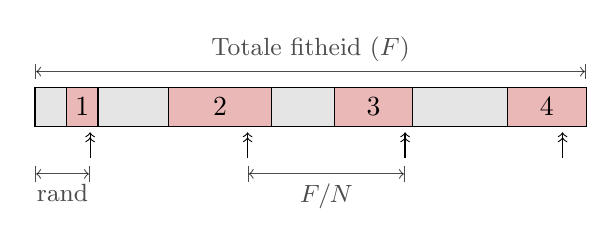
\begin{tikzpicture}

\foreach \x in {0.7,2.7,4.7,6.7}
    \draw[->>] (\x cm,-0.4cm) -- (\x cm,-2pt);

\draw[fill=black,fill opacity=0.1] (0,0) rectangle (7,0.5);

\foreach \x in {0.4,0.8,1.7,3,3.8,4.8,6}
    \draw (\x cm,0pt) -- (\x cm,0.5);

\draw[fill=mymark] (0.4,0) rectangle node {1} (0.8,0.5);
\draw[fill=mymark] (1.7,0) rectangle node {2} (3.0,0.5);
\draw[fill=mymark] (3.8,0) rectangle node {3} (4.8,0.5);
\draw[fill=mymark] (6.0,0) rectangle node {4} (7.0,0.5);

\draw[|<->|,black,opacity=0.7] (0,0.7) -- node[above] {\small Totale fitheid ($F$)} (7,0.7);
\draw[|<->|,black,opacity=0.7] (2.7,-0.6) -- node[below] {\small $F/N$} (4.7,-0.6);
\draw[|<->|,black,opacity=0.7] (0,-0.6) -- node[below] {\small rand} (0.7,-0.6);

%node[anchor=north] {\x};
\end{tikzpicture}
\caption{Visualisatie Stochastic Universal Sampling}
\label{fig:SUS}
\end{figure}
\end{center}


\subsubsection{Algoritme}
Het algoritme die het voorgaande idee implementeert heeft volgende vorm:
	\begin{algorithm}[H]
	 	\caption{Stochastic Universal Sampeling}
		\begin{algorithmic}
		\Require 
			\State $P$, te grote lijst van individuën 
			\State $N_l$, gewenste aantal individuen
		\Ensure returnt een lijst van gekozen individuen
		\Function{SUS}{$P$,$N_t$}
		\State Q $\gets \emptyset$
		\State total $\gets \sum_{x \in P} f(x)$ 
		\State size $\gets \frac{\text{total}}{N_l}$
		\State offset $\gets$ arbitraire waarde uit $\left\lbrack 0,\text{size} \right\rbrack$
		\State $t \gets$ offset
		\For{\textbf{each} $p \in P$} 
		\State $t = t-p.$fitness
		\If{$t<0$}
			\State $Q = Q \cup \lbrace p \rbrace$
			\State $t = t+$offset
		\EndIf
		\EndFor		
		\State \Return i
		\EndFunction

		
		\end{algorithmic}
		\label{alg:SUS}
	\end{algorithm}		
% subsubsection  (end)

\subsubsection{Complexiteit}
\label{ssub:SUSComplexity}
We moeten nagenoeg alle individuen in de populatie overopen. We kunnen dus stellen dat de complexiteit $ \Theta(\abs{P})$ is, met $\abs{P}$ de grootte van de populatie. Nu is $\abs{P}$ geen argument van ons programma. Dus bekomen we een complexiteit van \[T(n) = \Theta(1)\]
% subsubsection  (end)

\subsubsection{Alternatief}
\label{sec:positiveTournament}
Een alternatief bestaat er in tournament selcetion te gebruiken zoals in Algoritme~\ref{alg:tournament} uit sectie~\ref{sub:tournament}. Hierbij moeten we natuurlijk wel groter dan gebruiken in plaats van kleiner dan om meer kans te geven aan betere individuen. De complexiteit hiervan is  \[T(n) = \Theta(\abs{P} \cdot P_M) = \Theta(1)\]

%\section{Bronnen}
Er moet vermeld worden dat het \texttt{icosagon.poly} bestand afkomstig is van Jonathan Peck. We hebben dit bestand uitgewisseld om een andere figuur dan het gegeven vierkant te hebben samen met een notie van de maximale fitheid voor 50 punten in deze figuur. Code is er natuurlijk niet uitgewisseld.

\begin{thebibliography}{9}

\bibitem{lamport94}
  Haupt, Randy L., and Sue Ellen Haupt. ``Practical genetic algorithms.'' (2004).

\bibitem{baker85}
Baker, James Edward. "Adaptive selection methods for genetic algorithms." Proceedings of an International Conference on Genetic Algorithms and their applications. 1985.

\bibitem{parra9748125}
Pit, Laurens Jan. "Parallel genetic algorithms." MS (Computer Sci.) Dissertation (1995).

\bibitem{cuofiezafm}
Brinkmann, Gunnar. "Datastructuren en Algoritmen III, 2014." Cursus (2014)

\bibitem{MPIDOC}
University of Tennessee, "MPI: A Message-Passing Interface Standard" Online PDF. http://www.mpi-forum.org/docs/mpi-3.0/mpi30-report.pdf (2012)



\end{thebibliography}
\end{document}
%\documentclass[11pt,a4paper]{article}
\usepackage[utf8]{inputenc}
\usepackage[dutch]{babel}
\usepackage{pgfplots}
\usepgfplotslibrary{units}
\usepackage{float}
\usepackage{amsmath,amsthm}
\usepackage{amsfonts}
\usepackage{amssymb}
\usepackage[left=2cm,right=2cm,top=2.5cm,bottom=2cm]{geometry}
\usepackage{graphicx}
\usepackage{multicol}
\usepackage{enumerate}
\usepackage{fancyhdr}
\pagestyle{fancy}
\usepackage{algorithm}
\usepackage{algpseudocode}
\usepackage{pgfplots}
\usepackage{multirow}
\usepackage{tikz}
\usetikzlibrary{calc}

\floatname{algorithm}{Algoritme}


\usepackage[font=small,labelfont=bf]{caption}
\captionsetup[table]{aboveskip=-0.8em}
\captionsetup[table]{belowskip=-0.7pt}


\lhead {DAIII Project: punten plaatsen} 
\chead{BAZ(~ \thepage ~ )NGA} 
\rhead{Robbert Gurdeep Singh}


\cfoot{} % get rid of the page number 

\usepackage{hyperref}
\usepackage{chngcntr}
\counterwithin*{section}{part}
\counterwithin{algorithm}{section}
\counterwithin{table}{section}
\counterwithin{figure}{section}

\hypersetup{
    colorlinks=false,
    pdfborder={0 0 0},
}

\author{Robbert Gurdeep Singh}
\title{{Project Algoritmen en datastructuren III}\\ \Huge Genetische algoritmen}
%\date{}



\pgfplotsset{compat=1.8}


\newcommand{\drawGraph}[4]{
\begin{tikzpicture}
\begin{axis}[scale only axis, 
	%x-as	
    xmin=0,
	xlabel=#1,	
	%y-as
	ylabel=#2,
	ymin=0,
	%Style
	height=5em,width=.37\textwidth,
	enlargelimits=0.05,
	grid=major,	legend pos=south east
]
#3
\end{axis}
\end{tikzpicture}
}


\newcommand{\lxaxis}[3]{\begin{tikzpicture}
\begin{axis}[scale only axis, 
cycle list name=exotic,
    xmode=log,
    log ticks with fixed point,
	%x-as	
	xlabel=#2,	
	%y-as
	ylabel=#1,
	ymin=0,
	%Style
	height=5em,width=.37\textwidth,
	enlargelimits=0.05,
	grid=major,	legend pos=south east
]
#3

\end{axis}
\end{tikzpicture}}

\newcommand{\rlxaxis}[3]{\begin{tikzpicture}
\begin{axis}[scale only axis, 
cycle list name=exotic,
    xmode=log,
    log ticks with fixed point,
	%x-as	
	xlabel=#2,	
	%y-as
	ylabel=#1,
	%Style
	height=5em,width=.37\textwidth,
	enlargelimits=0.05,
	grid=major,	legend pos=south east
]
#3

\end{axis}
\end{tikzpicture}}

\newcommand{\nxaxis}[3]{\begin{tikzpicture}
\begin{axis}[scale only axis,
cycle list name=exotic, 
	%x-as	
    xmin=0,
	xlabel=#2,	
	%y-as
	ylabel=#1,
	ymin=0,
	%Style
	height=5em,width=.37\textwidth,
	enlargelimits=0.05,
	grid=major,	legend pos=south east
]
#3

\end{axis}
\end{tikzpicture}}


\newcommand{\rnxaxis}[3]{\begin{tikzpicture}
\begin{axis}[scale only axis, 
cycle list name=exotic,
	%x-as	
    xmin=0,
	xlabel=#2,	
	%y-as
	ylabel=#1,
	%Style
	height=5em,width=.37\textwidth,
	enlargelimits=0.05,
	grid=major,	legend pos=south east
]
#3

\end{axis}
\end{tikzpicture}}

\newcommand{\itemMB}[1]{
	\item[$\boldsymbol{#1}$:]
}




\newcommand{\abs}[1]{
	\lvert #1 \rvert
}

\newcommand{\addploti}[1]{\addplot table [y=i, x=testValue, col sep=comma] {../../tests/param_results/#1.log};}
\newcommand{\addplotf}[1]{\addplot table [y=f, x=testValue, col sep=comma] {../../tests/param_results/#1.log};}
\newcommand{\addplott}[1]{\addplot table [y=t, x=testValue, col sep=comma] {../../tests/param_results/#1.log};}

\definecolor{mymark}{HTML}{EBB8B8}

\begin{document}

\twocolumn[\begin{@twocolumnfalse}
    \maketitle
\end{@twocolumnfalse}]
\subsection{Mutation}
\label{sub:Mutation}
We willen er voor zorgend dat de diversiteit in de samenleving niet verdwijnt. Daarom zullen we kleine afwijkingen introduceren. Mochten we dit niet doen, dan zouden we nooit andere punten kunnen krijgen dan deze die initieel gekozen zijn.

\subsubsection{Idee}
Nadat er een kind gevormd is zullen we het met een bepaalde kans laten veranderen. Dat is dus dat er 1 punt lichtjes wordt verplaatst. Deze verplaatsing doen we door een nieuw punt te kiezen in de omgeving van het oorspronkelijk punt. Als dit gerandomiseerd punt buiten de figuur valt, proberen we het opnieuw met een kleinere omgeving.

\subsubsection{Algoritme}
\label{ssub:MutationAlgorithm}
Het algoritme die het voorgaande idee implementeert wordt beschreven in \ref{alg:Mutation}.
	\begin{algorithm}[H]
	 	\caption{Mutatie}
		\begin{algorithmic}
		\Require \State $I$, een individu \State $poly$ de veelhoek
		\Ensure $I$ is mischien gemuteeerd 
		
		\If{\texttt{rand() \% MUTATION\_1\_IN} = 0}
			\State $P \gets$ arbitrair punt van $I$ 
			\State $r \gets$ diameter van poly / \texttt{MUTATION\_DELTA}
			\Repeat 
			\State kies $(x_{new},y_{new}) \in \mathring{B}(P,r)$
			\State $r \gets r/2$
			\Until{$(x_{new},y_{new}) \in poly$}
		\EndIf		
		\end{algorithmic}
		\label{alg:Mutation}
	\end{algorithm}		
% subsubsection  (end)
Hierbij is de ``diameter van poly'' de maximale afstand tussen 2 punten van de convexe veelhoek.

\subsubsection{Implementatie}
\label{ssub:MutationImplementation}
De diagonaal die we in sectie \ref{ssub:MutationAlgorithm} beschouwen, word bij de implementatie zeer ruw benaderd door de diagonaal van het omgestoten vierkant te bepalen.

De implementatie is terug te vinden in \\
\texttt{do\_mutation()} van \texttt{genetic\_base.c}
% subsubsection  (end)

\subsubsection{Complexiteit}
\label{ssub:MutationComplexity}
Het kiezen van een nieuw punt is een operatie die in constante tijd kan gebeuren. Het nagaan dat het in de figuur ligt vraagt echter $\Theta(z)$ met $z$ het aantal zijden in de veelhoek\footnote{Zie Subsectie \ref{sub:algo-pt-in-poly}}.
% subsubsection  (end)

%\section{Bronnen}
Er moet vermeld worden dat het \texttt{icosagon.poly} bestand afkomstig is van Jonathan Peck. We hebben dit bestand uitgewisseld om een andere figuur dan het gegeven vierkant te hebben samen met een notie van de maximale fitheid voor 50 punten in deze figuur. Code is er natuurlijk niet uitgewisseld.

\begin{thebibliography}{9}

\bibitem{lamport94}
  Haupt, Randy L., and Sue Ellen Haupt. ``Practical genetic algorithms.'' (2004).

\bibitem{baker85}
Baker, James Edward. "Adaptive selection methods for genetic algorithms." Proceedings of an International Conference on Genetic Algorithms and their applications. 1985.

\bibitem{parra9748125}
Pit, Laurens Jan. "Parallel genetic algorithms." MS (Computer Sci.) Dissertation (1995).

\bibitem{cuofiezafm}
Brinkmann, Gunnar. "Datastructuren en Algoritmen III, 2014." Cursus (2014)

\bibitem{MPIDOC}
University of Tennessee, "MPI: A Message-Passing Interface Standard" Online PDF. http://www.mpi-forum.org/docs/mpi-3.0/mpi30-report.pdf (2012)



\end{thebibliography}
\end{document}
%\documentclass[11pt,a4paper]{article}
\usepackage[utf8]{inputenc}
\usepackage[dutch]{babel}
\usepackage{pgfplots}
\usepgfplotslibrary{units}
\usepackage{float}
\usepackage{amsmath,amsthm}
\usepackage{amsfonts}
\usepackage{amssymb}
\usepackage[left=2cm,right=2cm,top=2.5cm,bottom=2cm]{geometry}
\usepackage{graphicx}
\usepackage{multicol}
\usepackage{enumerate}
\usepackage{fancyhdr}
\pagestyle{fancy}
\usepackage{algorithm}
\usepackage{algpseudocode}
\usepackage{pgfplots}
\usepackage{multirow}
\usepackage{tikz}
\usetikzlibrary{calc}

\floatname{algorithm}{Algoritme}


\usepackage[font=small,labelfont=bf]{caption}
\captionsetup[table]{aboveskip=-0.8em}
\captionsetup[table]{belowskip=-0.7pt}


\lhead {DAIII Project: punten plaatsen} 
\chead{BAZ(~ \thepage ~ )NGA} 
\rhead{Robbert Gurdeep Singh}


\cfoot{} % get rid of the page number 

\usepackage{hyperref}
\usepackage{chngcntr}
\counterwithin*{section}{part}
\counterwithin{algorithm}{section}
\counterwithin{table}{section}
\counterwithin{figure}{section}

\hypersetup{
    colorlinks=false,
    pdfborder={0 0 0},
}

\author{Robbert Gurdeep Singh}
\title{{Project Algoritmen en datastructuren III}\\ \Huge Genetische algoritmen}
%\date{}



\pgfplotsset{compat=1.8}


\newcommand{\drawGraph}[4]{
\begin{tikzpicture}
\begin{axis}[scale only axis, 
	%x-as	
    xmin=0,
	xlabel=#1,	
	%y-as
	ylabel=#2,
	ymin=0,
	%Style
	height=5em,width=.37\textwidth,
	enlargelimits=0.05,
	grid=major,	legend pos=south east
]
#3
\end{axis}
\end{tikzpicture}
}


\newcommand{\lxaxis}[3]{\begin{tikzpicture}
\begin{axis}[scale only axis, 
cycle list name=exotic,
    xmode=log,
    log ticks with fixed point,
	%x-as	
	xlabel=#2,	
	%y-as
	ylabel=#1,
	ymin=0,
	%Style
	height=5em,width=.37\textwidth,
	enlargelimits=0.05,
	grid=major,	legend pos=south east
]
#3

\end{axis}
\end{tikzpicture}}

\newcommand{\rlxaxis}[3]{\begin{tikzpicture}
\begin{axis}[scale only axis, 
cycle list name=exotic,
    xmode=log,
    log ticks with fixed point,
	%x-as	
	xlabel=#2,	
	%y-as
	ylabel=#1,
	%Style
	height=5em,width=.37\textwidth,
	enlargelimits=0.05,
	grid=major,	legend pos=south east
]
#3

\end{axis}
\end{tikzpicture}}

\newcommand{\nxaxis}[3]{\begin{tikzpicture}
\begin{axis}[scale only axis,
cycle list name=exotic, 
	%x-as	
    xmin=0,
	xlabel=#2,	
	%y-as
	ylabel=#1,
	ymin=0,
	%Style
	height=5em,width=.37\textwidth,
	enlargelimits=0.05,
	grid=major,	legend pos=south east
]
#3

\end{axis}
\end{tikzpicture}}


\newcommand{\rnxaxis}[3]{\begin{tikzpicture}
\begin{axis}[scale only axis, 
cycle list name=exotic,
	%x-as	
    xmin=0,
	xlabel=#2,	
	%y-as
	ylabel=#1,
	%Style
	height=5em,width=.37\textwidth,
	enlargelimits=0.05,
	grid=major,	legend pos=south east
]
#3

\end{axis}
\end{tikzpicture}}

\newcommand{\itemMB}[1]{
	\item[$\boldsymbol{#1}$:]
}




\newcommand{\abs}[1]{
	\lvert #1 \rvert
}

\newcommand{\addploti}[1]{\addplot table [y=i, x=testValue, col sep=comma] {../../tests/param_results/#1.log};}
\newcommand{\addplotf}[1]{\addplot table [y=f, x=testValue, col sep=comma] {../../tests/param_results/#1.log};}
\newcommand{\addplott}[1]{\addplot table [y=t, x=testValue, col sep=comma] {../../tests/param_results/#1.log};}

\definecolor{mymark}{HTML}{EBB8B8}

\begin{document}

\twocolumn[\begin{@twocolumnfalse}
    \maketitle
\end{@twocolumnfalse}]
\subsection{Crossover}
\label{sub:crossover}
Als 2 individuen geselecteerd zijn om te paren, dan moeten wij daaruit een kind creëren dat eigenschappen van beide ouders bevat. Dit doen we door het eerste deel van de ene ouder samen te stellen met het tweede deel van de andere ouder (en omgekeerd voor het genereren van een 2de kind). Deze aanpak staat beschreven in Algoritme~\ref{alg:crossover-1point}.
Alternatief kunnen we er ook voor kiezen om een willekeurig aantal keer te wissen (Algoritme \ref{alg:crossover-random}).
\subsubsection{Algoritme}
	\begin{algorithm}[H]
	 	\caption{1-point Crossover}
		\begin{algorithmic}
		\Require \State $mama, papa$ de ouders \State $n$ het aantal te plaatsen punten
		\Ensure $kind$ is een nieuw kind dat genetisch gelijkend is met de ouders
		\State $r \gets$ arbitrair getal in $\lbrace 1, \dots , n-2\rbrace$
		\For{i \textbf{from} 0 \textbf{to} $r$}
			\State $kind$.punten[$i$] $\gets mama$.punten[$i$]
		\EndFor
		\For{i \textbf{from} $r+1$ \textbf{to} $n-1$}
			\State $kind$.punten[$i$] $\gets papa$.punten[$i$]
		\EndFor
		\end{algorithmic}
		\label{alg:crossover-1point}
	\end{algorithm}		

	\begin{algorithm}[H]
	 	\caption{random Crossover}
		\begin{algorithmic}
		\Require \State $mama, papa$ de ouders \State $n$ het aantal te plaatsen punten
		\Ensure $kind$ is een nieuw kind dat genetisch gelijkend is met de ouders
		
		\State $r \gets$ arbitrair getal in $\lbrace 1, \dots , n-2\rbrace$
		\For{i \textbf{from} 0 \textbf{to} $n-1$}
		\State $oud$ $\gets$ arbitrare waarde uit $\lbrace mama, papa \rbrace$
		\State $kind$.punten[$i$] $\gets oud$.punten[$i$]
			
		\EndFor

		\end{algorithmic}
		\label{alg:crossover-random}
	\end{algorithm}		



\subsubsection{Complexiteit}
\label{sub:alg_crossover_compl}
Een crossover kopieert $n$ waarden. Het is dus \[T(n)=\Theta(n)\]


% subsection  (end)


\subsubsection{Implementatie}
Het bestand \texttt{genetic\_base.c} bevat de implementatie van Algoritme \ref{alg:crossover-1point} en \ref{alg:crossover-random} in de functie 
\\ \texttt{do\_crossover()}. 
Het bestand bevat beide implementaties, bij compilatie kan er tussen beide gekozen worden door we waarde van \\ \texttt{RANDOM\_CROSSOVER} in te stellen met de \texttt{-D} vlag van de compiler. Standaard staat deze waarde ingesteld op 1-point, de reden hiervoor vind u in sectie \ref{ssub:crossover_type}.


%\section{Bronnen}
Er moet vermeld worden dat het \texttt{icosagon.poly} bestand afkomstig is van Jonathan Peck. We hebben dit bestand uitgewisseld om een andere figuur dan het gegeven vierkant te hebben samen met een notie van de maximale fitheid voor 50 punten in deze figuur. Code is er natuurlijk niet uitgewisseld.

\begin{thebibliography}{9}

\bibitem{lamport94}
  Haupt, Randy L., and Sue Ellen Haupt. ``Practical genetic algorithms.'' (2004).

\bibitem{baker85}
Baker, James Edward. "Adaptive selection methods for genetic algorithms." Proceedings of an International Conference on Genetic Algorithms and their applications. 1985.

\bibitem{parra9748125}
Pit, Laurens Jan. "Parallel genetic algorithms." MS (Computer Sci.) Dissertation (1995).

\bibitem{cuofiezafm}
Brinkmann, Gunnar. "Datastructuren en Algoritmen III, 2014." Cursus (2014)

\bibitem{MPIDOC}
University of Tennessee, "MPI: A Message-Passing Interface Standard" Online PDF. http://www.mpi-forum.org/docs/mpi-3.0/mpi30-report.pdf (2012)



\end{thebibliography}
\end{document}
%\documentclass[11pt,a4paper]{article}
\usepackage[utf8]{inputenc}
\usepackage[dutch]{babel}
\usepackage{pgfplots}
\usepgfplotslibrary{units}
\usepackage{float}
\usepackage{amsmath,amsthm}
\usepackage{amsfonts}
\usepackage{amssymb}
\usepackage[left=2cm,right=2cm,top=2.5cm,bottom=2cm]{geometry}
\usepackage{graphicx}
\usepackage{multicol}
\usepackage{enumerate}
\usepackage{fancyhdr}
\pagestyle{fancy}
\usepackage{algorithm}
\usepackage{algpseudocode}
\usepackage{pgfplots}
\usepackage{multirow}
\usepackage{tikz}
\usetikzlibrary{calc}

\floatname{algorithm}{Algoritme}


\usepackage[font=small,labelfont=bf]{caption}
\captionsetup[table]{aboveskip=-0.8em}
\captionsetup[table]{belowskip=-0.7pt}


\lhead {DAIII Project: punten plaatsen} 
\chead{BAZ(~ \thepage ~ )NGA} 
\rhead{Robbert Gurdeep Singh}


\cfoot{} % get rid of the page number 

\usepackage{hyperref}
\usepackage{chngcntr}
\counterwithin*{section}{part}
\counterwithin{algorithm}{section}
\counterwithin{table}{section}
\counterwithin{figure}{section}

\hypersetup{
    colorlinks=false,
    pdfborder={0 0 0},
}

\author{Robbert Gurdeep Singh}
\title{{Project Algoritmen en datastructuren III}\\ \Huge Genetische algoritmen}
%\date{}



\pgfplotsset{compat=1.8}


\newcommand{\drawGraph}[4]{
\begin{tikzpicture}
\begin{axis}[scale only axis, 
	%x-as	
    xmin=0,
	xlabel=#1,	
	%y-as
	ylabel=#2,
	ymin=0,
	%Style
	height=5em,width=.37\textwidth,
	enlargelimits=0.05,
	grid=major,	legend pos=south east
]
#3
\end{axis}
\end{tikzpicture}
}


\newcommand{\lxaxis}[3]{\begin{tikzpicture}
\begin{axis}[scale only axis, 
cycle list name=exotic,
    xmode=log,
    log ticks with fixed point,
	%x-as	
	xlabel=#2,	
	%y-as
	ylabel=#1,
	ymin=0,
	%Style
	height=5em,width=.37\textwidth,
	enlargelimits=0.05,
	grid=major,	legend pos=south east
]
#3

\end{axis}
\end{tikzpicture}}

\newcommand{\rlxaxis}[3]{\begin{tikzpicture}
\begin{axis}[scale only axis, 
cycle list name=exotic,
    xmode=log,
    log ticks with fixed point,
	%x-as	
	xlabel=#2,	
	%y-as
	ylabel=#1,
	%Style
	height=5em,width=.37\textwidth,
	enlargelimits=0.05,
	grid=major,	legend pos=south east
]
#3

\end{axis}
\end{tikzpicture}}

\newcommand{\nxaxis}[3]{\begin{tikzpicture}
\begin{axis}[scale only axis,
cycle list name=exotic, 
	%x-as	
    xmin=0,
	xlabel=#2,	
	%y-as
	ylabel=#1,
	ymin=0,
	%Style
	height=5em,width=.37\textwidth,
	enlargelimits=0.05,
	grid=major,	legend pos=south east
]
#3

\end{axis}
\end{tikzpicture}}


\newcommand{\rnxaxis}[3]{\begin{tikzpicture}
\begin{axis}[scale only axis, 
cycle list name=exotic,
	%x-as	
    xmin=0,
	xlabel=#2,	
	%y-as
	ylabel=#1,
	%Style
	height=5em,width=.37\textwidth,
	enlargelimits=0.05,
	grid=major,	legend pos=south east
]
#3

\end{axis}
\end{tikzpicture}}

\newcommand{\itemMB}[1]{
	\item[$\boldsymbol{#1}$:]
}




\newcommand{\abs}[1]{
	\lvert #1 \rvert
}

\newcommand{\addploti}[1]{\addplot table [y=i, x=testValue, col sep=comma] {../../tests/param_results/#1.log};}
\newcommand{\addplotf}[1]{\addplot table [y=f, x=testValue, col sep=comma] {../../tests/param_results/#1.log};}
\newcommand{\addplott}[1]{\addplot table [y=t, x=testValue, col sep=comma] {../../tests/param_results/#1.log};}

\definecolor{mymark}{HTML}{EBB8B8}

\begin{document}

\twocolumn[\begin{@twocolumnfalse}
    \maketitle
\end{@twocolumnfalse}]
\subsection{Stopvoorwaarde}
\label{ssub:stop_cond}
We moeten nu nog een voorwaarde opstellen om te stoppen met itereren. We willen pas stoppen als we er nagenoeg zeker van zijn dat er geen verbetering meer zal zijn.
\subsubsection{Idee}
We willen een waarde hebben die een maat is voor de grootte van recente verandering van de maximale fitheid in de populatie. Hiervoor zouden we een exponentieel lopend gemiddelde kunnen bijhouden van de verandering van de maximale fitheid per iteratie. Als we de maximale fitheid na de $i$-de iteratie $\bar f(i)$ noemen,dan kunnen we zo'n exponenteel lopend gemiddelde als volgt defineeren:
\[\Delta_i = \bar f(i) - \bar f(i-1)\]
\[g(i) =  \Delta_i \cdot (1-\alpha) + g(i-1)\cdot \alpha\]
met $\alpha$ een weegfactor\footnote{In ons project is dit \texttt{WEIGHTING\_DECREASE}; Zie Sectie~\ref{sub:weightingFactor} voor een bespreking van de optimale waarde.} die in $\rbrack 0,1 \lbrack$.

Als we dit in expliciete vorm herschrijven zien we dat het verleden steeds minder waarde heeft.
\[g(i) = (1-\alpha) \sum^i_{j=0} \Delta_j \cdot \alpha^j + g(0)\cdot \alpha^{i+1}\]

We kunnen nu verwachten dat het niet meer veel zal verbeteren eens $g(i)$ nagenoeg nul\footnote{geimplementeerd als ``minder dan $10^{11}$''} is. Door $g(0)$ een hoge waarde te geven zorgen we er kunstmatig voor dat we een minimum aantal iteraties hebben. 
 
\subsubsection{Algoritme \& Implementatie}
Voor het beginnen van de iteraties houden we twee variabelen bij. Deze variabelen stellen de vorige maximale fitheid en de huidige waarde van $g(i)$ voor. Na elke iteratie herberekenen we die waarden. Eens $g(i)$ onder de treshhold valt stoppen we met itereren. Om het eindigen van het algoritme te verzekeren gebruiken we een bovengrens voor het aantal iteraties.
 
%\section{Bronnen}
Er moet vermeld worden dat het \texttt{icosagon.poly} bestand afkomstig is van Jonathan Peck. We hebben dit bestand uitgewisseld om een andere figuur dan het gegeven vierkant te hebben samen met een notie van de maximale fitheid voor 50 punten in deze figuur. Code is er natuurlijk niet uitgewisseld.

\begin{thebibliography}{9}

\bibitem{lamport94}
  Haupt, Randy L., and Sue Ellen Haupt. ``Practical genetic algorithms.'' (2004).

\bibitem{baker85}
Baker, James Edward. "Adaptive selection methods for genetic algorithms." Proceedings of an International Conference on Genetic Algorithms and their applications. 1985.

\bibitem{parra9748125}
Pit, Laurens Jan. "Parallel genetic algorithms." MS (Computer Sci.) Dissertation (1995).

\bibitem{cuofiezafm}
Brinkmann, Gunnar. "Datastructuren en Algoritmen III, 2014." Cursus (2014)

\bibitem{MPIDOC}
University of Tennessee, "MPI: A Message-Passing Interface Standard" Online PDF. http://www.mpi-forum.org/docs/mpi-3.0/mpi30-report.pdf (2012)



\end{thebibliography}
\end{document}
%\documentclass[11pt,a4paper]{article}
\usepackage[utf8]{inputenc}
\usepackage[dutch]{babel}
\usepackage{pgfplots}
\usepgfplotslibrary{units}
\usepackage{float}
\usepackage{amsmath,amsthm}
\usepackage{amsfonts}
\usepackage{amssymb}
\usepackage[left=2cm,right=2cm,top=2.5cm,bottom=2cm]{geometry}
\usepackage{graphicx}
\usepackage{multicol}
\usepackage{enumerate}
\usepackage{fancyhdr}
\pagestyle{fancy}
\usepackage{algorithm}
\usepackage{algpseudocode}
\usepackage{pgfplots}
\usepackage{multirow}
\usepackage{tikz}
\usetikzlibrary{calc}

\floatname{algorithm}{Algoritme}


\usepackage[font=small,labelfont=bf]{caption}
\captionsetup[table]{aboveskip=-0.8em}
\captionsetup[table]{belowskip=-0.7pt}


\lhead {DAIII Project: punten plaatsen} 
\chead{BAZ(~ \thepage ~ )NGA} 
\rhead{Robbert Gurdeep Singh}


\cfoot{} % get rid of the page number 

\usepackage{hyperref}
\usepackage{chngcntr}
\counterwithin*{section}{part}
\counterwithin{algorithm}{section}
\counterwithin{table}{section}
\counterwithin{figure}{section}

\hypersetup{
    colorlinks=false,
    pdfborder={0 0 0},
}

\author{Robbert Gurdeep Singh}
\title{{Project Algoritmen en datastructuren III}\\ \Huge Genetische algoritmen}
%\date{}



\pgfplotsset{compat=1.8}


\newcommand{\drawGraph}[4]{
\begin{tikzpicture}
\begin{axis}[scale only axis, 
	%x-as	
    xmin=0,
	xlabel=#1,	
	%y-as
	ylabel=#2,
	ymin=0,
	%Style
	height=5em,width=.37\textwidth,
	enlargelimits=0.05,
	grid=major,	legend pos=south east
]
#3
\end{axis}
\end{tikzpicture}
}


\newcommand{\lxaxis}[3]{\begin{tikzpicture}
\begin{axis}[scale only axis, 
cycle list name=exotic,
    xmode=log,
    log ticks with fixed point,
	%x-as	
	xlabel=#2,	
	%y-as
	ylabel=#1,
	ymin=0,
	%Style
	height=5em,width=.37\textwidth,
	enlargelimits=0.05,
	grid=major,	legend pos=south east
]
#3

\end{axis}
\end{tikzpicture}}

\newcommand{\rlxaxis}[3]{\begin{tikzpicture}
\begin{axis}[scale only axis, 
cycle list name=exotic,
    xmode=log,
    log ticks with fixed point,
	%x-as	
	xlabel=#2,	
	%y-as
	ylabel=#1,
	%Style
	height=5em,width=.37\textwidth,
	enlargelimits=0.05,
	grid=major,	legend pos=south east
]
#3

\end{axis}
\end{tikzpicture}}

\newcommand{\nxaxis}[3]{\begin{tikzpicture}
\begin{axis}[scale only axis,
cycle list name=exotic, 
	%x-as	
    xmin=0,
	xlabel=#2,	
	%y-as
	ylabel=#1,
	ymin=0,
	%Style
	height=5em,width=.37\textwidth,
	enlargelimits=0.05,
	grid=major,	legend pos=south east
]
#3

\end{axis}
\end{tikzpicture}}


\newcommand{\rnxaxis}[3]{\begin{tikzpicture}
\begin{axis}[scale only axis, 
cycle list name=exotic,
	%x-as	
    xmin=0,
	xlabel=#2,	
	%y-as
	ylabel=#1,
	%Style
	height=5em,width=.37\textwidth,
	enlargelimits=0.05,
	grid=major,	legend pos=south east
]
#3

\end{axis}
\end{tikzpicture}}

\newcommand{\itemMB}[1]{
	\item[$\boldsymbol{#1}$:]
}




\newcommand{\abs}[1]{
	\lvert #1 \rvert
}

\newcommand{\addploti}[1]{\addplot table [y=i, x=testValue, col sep=comma] {../../tests/param_results/#1.log};}
\newcommand{\addplotf}[1]{\addplot table [y=f, x=testValue, col sep=comma] {../../tests/param_results/#1.log};}
\newcommand{\addplott}[1]{\addplot table [y=t, x=testValue, col sep=comma] {../../tests/param_results/#1.log};}

\definecolor{mymark}{HTML}{EBB8B8}

\begin{document}

\twocolumn[\begin{@twocolumnfalse}
    \maketitle
\end{@twocolumnfalse}]
\subsection{Het genetisch algoritme}
\label{ssub:genetic}
Nu we alle onderdelen van het genetisch algoritme hebben besproken kunnen we het samenbrengen tot een geheel.

\subsubsection{Algoritme}
	\begin{algorithm}[H]
	 	\caption{Het genetisch algoritme}
		\begin{algorithmic}
		\Require $n$, het aantal te plaatsen punten
		\Ensure een goede benadeering van een oplossing die aan de voorwaarden van een oplossing voldoet wordt eteeruggegeven
		\Function{darwinsPoints}{}
		\State $P \gets $ $N_p$ random individuen 
		\Comment Sec \ref{ssub:rand_generation}
		\While{niet stopconditie} 
		\Comment Sec \ref{ssub:stop_cond}
			\State $L \gets$ \Call{selectLovers}{$N_l$} 
			\Comment Sec \ref{sec:positiveTournament}
			\For{$i\gets 0 \dots \lfloor \abs{L}/2 \rfloor$ }
				\State Maak 2 kinderen met ouders 
				\State $L\lbrack2i\rbrack$ en  $L\lbrack2i+1\rbrack$ en voeg ze 
				\State toe aan $P$ 
				\Comment Sec \ref{sub:crossover}
				\State Bereken fitheid kinden
			\EndFor
			\State \Call{tournament}{$P$,$N_p$} 
			\Comment Sec \ref{sub:tournament}
		\EndWhile 
		\State \Return  $\displaystyle opl \in \lbrace x \in P \mid f(x) = \max_{y\in P}{f(y)}  \rbrace$
		\EndFunction
		\end{algorithmic}
		\label{alg:genetic}
	\end{algorithm}		
    Merk op dat we in dit algoritme tournament selection gebruikt voor zowel het selecteren van wie sterft als voor het selecteren wie seks heeft. We hebben de verklaring hiervoor geformuleerd in Sectie~\ref{sub:algLoverSelection}. 
\subsubsection{Complexiteisanalyse}
  Overlopen de stappen in Algoritme~\ref{alg:genetic} om de complexiteit te bepalen:
\begin{enumerate}
	\itembf{Random generatie} Sectie~\ref{ssub:rand_generation} geeft ons:\\ $T_{gen}(n)=\Theta(N_p\cdot n) = \Theta(n)$ 
	\itembf{Iteraties}
		\begin{enumerate}
			\itembf{Lover selection} \\$T(n)= \cdot P_M \cdot N_p = \Theta(1)$ 
			\itembf{Crossover} Uit sectie \ref{sub:alg_crossover_compl}\\$T_{\text{1}}(n)= \Theta(N_l\cdot n) = \Theta(n)$
			\itembf{Fitheid kinderen berekenen} \\$T_{\text{1}}(n)= \Theta(n^2)$
			\itembf{Tournament Selection} \\$T(n)= \Theta(N_p\cdot P_M) = \Theta(1)$
		\end{enumerate}
	\itembf{Beste teruggeven}
		\\Alles overlopen dus $T(n)=\Theta(N_p)=\Theta(1)$
\end{enumerate}

In de 2de grafiek van figuur \ref{graf:algLoverSelection} op pagina \pageref{graf:algLoverSelection} zien we dat het aantal iteraties $\Theta(n)$ is. We komen dus uit op een totale complexiteit van \[T(n)=\Theta\left(n^3\right)\]

Er dient opgemerkt te worden dat het aantal iteraties begrensd is in onze implementatie. Dus als $n$ zo groot is dat het maximaal aantal iteraties wordt overschreden, dan in de complexiteit $\Theta{n^2}$.

%\section{Bronnen}
Er moet vermeld worden dat het \texttt{icosagon.poly} bestand afkomstig is van Jonathan Peck. We hebben dit bestand uitgewisseld om een andere figuur dan het gegeven vierkant te hebben samen met een notie van de maximale fitheid voor 50 punten in deze figuur. Code is er natuurlijk niet uitgewisseld.

\begin{thebibliography}{9}

\bibitem{lamport94}
  Haupt, Randy L., and Sue Ellen Haupt. ``Practical genetic algorithms.'' (2004).

\bibitem{baker85}
Baker, James Edward. "Adaptive selection methods for genetic algorithms." Proceedings of an International Conference on Genetic Algorithms and their applications. 1985.

\bibitem{parra9748125}
Pit, Laurens Jan. "Parallel genetic algorithms." MS (Computer Sci.) Dissertation (1995).

\bibitem{cuofiezafm}
Brinkmann, Gunnar. "Datastructuren en Algoritmen III, 2014." Cursus (2014)

\bibitem{MPIDOC}
University of Tennessee, "MPI: A Message-Passing Interface Standard" Online PDF. http://www.mpi-forum.org/docs/mpi-3.0/mpi30-report.pdf (2012)



\end{thebibliography}
\end{document}

%\documentclass[11pt,a4paper]{article}
\usepackage[utf8]{inputenc}
\usepackage[dutch]{babel}
\usepackage{pgfplots}
\usepgfplotslibrary{units}
\usepackage{float}
\usepackage{amsmath,amsthm}
\usepackage{amsfonts}
\usepackage{amssymb}
\usepackage[left=2cm,right=2cm,top=2.5cm,bottom=2cm]{geometry}
\usepackage{graphicx}
\usepackage{multicol}
\usepackage{enumerate}
\usepackage{fancyhdr}
\pagestyle{fancy}
\usepackage{algorithm}
\usepackage{algpseudocode}
\usepackage{pgfplots}
\usepackage{multirow}
\usepackage{tikz}
\usetikzlibrary{calc}

\floatname{algorithm}{Algoritme}


\usepackage[font=small,labelfont=bf]{caption}
\captionsetup[table]{aboveskip=-0.8em}
\captionsetup[table]{belowskip=-0.7pt}


\lhead {DAIII Project: punten plaatsen} 
\chead{BAZ(~ \thepage ~ )NGA} 
\rhead{Robbert Gurdeep Singh}


\cfoot{} % get rid of the page number 

\usepackage{hyperref}
\usepackage{chngcntr}
\counterwithin*{section}{part}
\counterwithin{algorithm}{section}
\counterwithin{table}{section}
\counterwithin{figure}{section}

\hypersetup{
    colorlinks=false,
    pdfborder={0 0 0},
}

\author{Robbert Gurdeep Singh}
\title{{Project Algoritmen en datastructuren III}\\ \Huge Genetische algoritmen}
%\date{}



\pgfplotsset{compat=1.8}


\newcommand{\drawGraph}[4]{
\begin{tikzpicture}
\begin{axis}[scale only axis, 
	%x-as	
    xmin=0,
	xlabel=#1,	
	%y-as
	ylabel=#2,
	ymin=0,
	%Style
	height=5em,width=.37\textwidth,
	enlargelimits=0.05,
	grid=major,	legend pos=south east
]
#3
\end{axis}
\end{tikzpicture}
}


\newcommand{\lxaxis}[3]{\begin{tikzpicture}
\begin{axis}[scale only axis, 
cycle list name=exotic,
    xmode=log,
    log ticks with fixed point,
	%x-as	
	xlabel=#2,	
	%y-as
	ylabel=#1,
	ymin=0,
	%Style
	height=5em,width=.37\textwidth,
	enlargelimits=0.05,
	grid=major,	legend pos=south east
]
#3

\end{axis}
\end{tikzpicture}}

\newcommand{\rlxaxis}[3]{\begin{tikzpicture}
\begin{axis}[scale only axis, 
cycle list name=exotic,
    xmode=log,
    log ticks with fixed point,
	%x-as	
	xlabel=#2,	
	%y-as
	ylabel=#1,
	%Style
	height=5em,width=.37\textwidth,
	enlargelimits=0.05,
	grid=major,	legend pos=south east
]
#3

\end{axis}
\end{tikzpicture}}

\newcommand{\nxaxis}[3]{\begin{tikzpicture}
\begin{axis}[scale only axis,
cycle list name=exotic, 
	%x-as	
    xmin=0,
	xlabel=#2,	
	%y-as
	ylabel=#1,
	ymin=0,
	%Style
	height=5em,width=.37\textwidth,
	enlargelimits=0.05,
	grid=major,	legend pos=south east
]
#3

\end{axis}
\end{tikzpicture}}


\newcommand{\rnxaxis}[3]{\begin{tikzpicture}
\begin{axis}[scale only axis, 
cycle list name=exotic,
	%x-as	
    xmin=0,
	xlabel=#2,	
	%y-as
	ylabel=#1,
	%Style
	height=5em,width=.37\textwidth,
	enlargelimits=0.05,
	grid=major,	legend pos=south east
]
#3

\end{axis}
\end{tikzpicture}}

\newcommand{\itemMB}[1]{
	\item[$\boldsymbol{#1}$:]
}




\newcommand{\abs}[1]{
	\lvert #1 \rvert
}

\newcommand{\addploti}[1]{\addplot table [y=i, x=testValue, col sep=comma] {../../tests/param_results/#1.log};}
\newcommand{\addplotf}[1]{\addplot table [y=f, x=testValue, col sep=comma] {../../tests/param_results/#1.log};}
\newcommand{\addplott}[1]{\addplot table [y=t, x=testValue, col sep=comma] {../../tests/param_results/#1.log};}

\definecolor{mymark}{HTML}{EBB8B8}

\begin{document}

\twocolumn[\begin{@twocolumnfalse}
    \maketitle
\end{@twocolumnfalse}]
\section{Parrameter Optimalisatie}
\subsection{Aantal individuën}
\begin{center}
\begin{figure}[H]
\rlxaxis{Fitness}{Aantal individus}{
	\addlegendentry{50 ptn}
	\addplotf{NUM_INDIVIDUS_vierkant_50};
	\addlegendentry{15 ptn}
	\addplotf{NUM_INDIVIDUS_soos_50};
	\addlegendentry{15 ptn}
	\addplotf{NUM_INDIVIDUS_icosagon_50};
}
\lxaxis{Iteraties}{Aantal individus}{
	\addlegendentry{50 ptn}
	\addploti{NUM_INDIVIDUS_vierkant_50};
	\addlegendentry{15 ptn}
	\addploti{NUM_INDIVIDUS_soos_50};
	\addlegendentry{\small 15 ptn}
}
\lxaxis{Tijd}{Aantal individus}{
	\addlegendentry{vierkant}
	\addplott{NUM_INDIVIDUS_vierkant_50};
	\addlegendentry{soos}
	\addplott{NUM_INDIVIDUS_soos_50};
}



\caption{Corelatie aantal individus op convergentie snelheid en kwaliteit}
\end{figure}
\end{center}

Dit zijn resultaten die wij a priori niet verachten. We zien een lokaal minium op 100. Dis is dus ook de ideale waarde



\subsection{Hoeveelheid seks}
\begin{center}
\begin{figure}[H]
\rnxaxis{Fitness}{Sekspercentage}{
	\addlegendentry{50 ptn}
	\addplotf{LOVER_PERCENT_vierkant_50};
	\addlegendentry{15 ptn}
	\addplotf{LOVER_PERCENT_soos_50};
	\addlegendentry{15 ptn}
	\addplotf{LOVER_PERCENT_icosagon_50};
}
\nxaxis{Iteraties}{Sekspercenntage}{
	\addlegendentry{50 ptn}
	\addploti{LOVER_PERCENT_vierkant_50};
	\addlegendentry{15 ptn}
	\addploti{LOVER_PERCENT_soos_50};
}
\nxaxis{Tijd}{Sekspercentage}{
	\addlegendentry{vierkant}
	\addplott{LOVER_PERCENT_vierkant_50};
	\addlegendentry{soos}
	\addplott{LOVER_PERCENT_soos_50};
}



\caption{Corelatie aantal individus op convergentie snelheid en kwaliteit}
\end{figure}
\end{center}

We zien dat we een afweging moeten maken tussen de hoeveellheid seks en de uitvoeringstijd.





\subsection{Hoeveelheid mutatie}
\begin{center}
\begin{figure}[H]
\rnxaxis{Fitness}{Delta}{
	\addlegendentry{50 ptn}
	\addplotf{MUTATION_DELTA_vierkant_50};
	\addlegendentry{15 ptn}
	\addplotf{MUTATION_DELTA_soos_50};
	\addlegendentry{15 ptn}
	\addplotf{MUTATION_DELTA_icosagon_50};
}
\nxaxis{Iteraties}{Delta}{
	\addlegendentry{50 ptn}
	\addploti{MUTATION_DELTA_vierkant_50};
	\addlegendentry{15 ptn}
	\addploti{MUTATION_DELTA_soos_50};
}
\nxaxis{Tijd (s)}{Delta}{
	\addlegendentry{vierkant}
	\addplott{MUTATION_DELTA_vierkant_50};
	\addlegendentry{soos}
	\addplott{MUTATION_DELTA_soos_50};
}



\caption{Corelatie aantal individus op convergentie snelheid en kwaliteit}
\end{figure}
\end{center}

Hoe groter de mutatie hoe beter. (MUTATION\_DELTA is omgekeerd)


\subsection{Mutatie kans}
\begin{center}
\begin{figure}[H]
\rlxaxis{Fitness}{Kans (1 op ...)}{
	\addlegendentry{50 ptn}
	\addplotf{MUTATION_1_IN_vierkant_50};
	\addlegendentry{15 ptn}
	\addplotf{MUTATION_1_IN_soos_50};
	\addlegendentry{15 ptn}
	\addplotf{MUTATION_1_IN_icosagon_50};
}
\lxaxis{Iteraties}{Kans (1 op ...)}{
	\addlegendentry{50 ptn}
	\addploti{MUTATION_1_IN_vierkant_50};
	\addlegendentry{15 ptn}
	\addploti{MUTATION_1_IN_soos_50};
}
\lxaxis{Tijd}{Kans (1 op ...)}{
	\addlegendentry{vierkant}
	\addplott{MUTATION_1_IN_vierkant_50};
	\addlegendentry{soos}
	\addplott{MUTATION_1_IN_soos_50};
}



\caption{Corelatie aantal individus op convergentie snelheid en kwaliteit}
\end{figure}
\end{center}

Hoe kleiner de kans hoe lager de fitness



\subsection{Selectie druk}
\begin{center}
\begin{figure}[H]
\nxaxis{Fitness}{Toernooigrootte}{
	\addlegendentry{50 ptn}
	\addplotf{SELECTION_PRESSURE_vierkant_50};
	\addlegendentry{15 ptn}
	\addplotf{SELECTION_PRESSURE_soos_50};
	\addlegendentry{15 ptn}
	\addplotf{SELECTION_PRESSURE_icosagon_50};
}
\nxaxis{Iteraties}{Toernooigrootte}{
	\addlegendentry{50 ptn}
	\addploti{SELECTION_PRESSURE_vierkant_50};
	\addlegendentry{15 ptn}
	\addploti{SELECTION_PRESSURE_soos_50};
}
\nxaxis{Tijd}{Toernooigrootte}{
	\addlegendentry{50 ptn}
	\addplott{SELECTION_PRESSURE_vierkant_50};
	\addlegendentry{15 ptn}
	\addplott{SELECTION_PRESSURE_soos_50};
}



\caption{Corelatie aantal individus op convergentie snelheid en kwaliteit}
\end{figure}
\end{center}

Hoe groter de mutd
%\section{Bronnen}
Er moet vermeld worden dat het \texttt{icosagon.poly} bestand afkomstig is van Jonathan Peck. We hebben dit bestand uitgewisseld om een andere figuur dan het gegeven vierkant te hebben samen met een notie van de maximale fitheid voor 50 punten in deze figuur. Code is er natuurlijk niet uitgewisseld.

\begin{thebibliography}{9}

\bibitem{lamport94}
  Haupt, Randy L., and Sue Ellen Haupt. ``Practical genetic algorithms.'' (2004).

\bibitem{baker85}
Baker, James Edward. "Adaptive selection methods for genetic algorithms." Proceedings of an International Conference on Genetic Algorithms and their applications. 1985.

\bibitem{parra9748125}
Pit, Laurens Jan. "Parallel genetic algorithms." MS (Computer Sci.) Dissertation (1995).

\bibitem{cuofiezafm}
Brinkmann, Gunnar. "Datastructuren en Algoritmen III, 2014." Cursus (2014)

\bibitem{MPIDOC}
University of Tennessee, "MPI: A Message-Passing Interface Standard" Online PDF. http://www.mpi-forum.org/docs/mpi-3.0/mpi30-report.pdf (2012)



\end{thebibliography}
\end{document}
%\documentclass[11pt,a4paper]{article}
\usepackage[utf8]{inputenc}
\usepackage[dutch]{babel}
\usepackage{pgfplots}
\usepgfplotslibrary{units}
\usepackage{float}
\usepackage{amsmath,amsthm}
\usepackage{amsfonts}
\usepackage{amssymb}
\usepackage[left=2cm,right=2cm,top=2.5cm,bottom=2cm]{geometry}
\usepackage{graphicx}
\usepackage{multicol}
\usepackage{enumerate}
\usepackage{fancyhdr}
\pagestyle{fancy}
\usepackage{algorithm}
\usepackage{algpseudocode}
\usepackage{pgfplots}
\usepackage{multirow}
\usepackage{tikz}
\usetikzlibrary{calc}

\floatname{algorithm}{Algoritme}


\usepackage[font=small,labelfont=bf]{caption}
\captionsetup[table]{aboveskip=-0.8em}
\captionsetup[table]{belowskip=-0.7pt}


\lhead {DAIII Project: punten plaatsen} 
\chead{BAZ(~ \thepage ~ )NGA} 
\rhead{Robbert Gurdeep Singh}


\cfoot{} % get rid of the page number 

\usepackage{hyperref}
\usepackage{chngcntr}
\counterwithin*{section}{part}
\counterwithin{algorithm}{section}
\counterwithin{table}{section}
\counterwithin{figure}{section}

\hypersetup{
    colorlinks=false,
    pdfborder={0 0 0},
}

\author{Robbert Gurdeep Singh}
\title{{Project Algoritmen en datastructuren III}\\ \Huge Genetische algoritmen}
%\date{}



\pgfplotsset{compat=1.8}


\newcommand{\drawGraph}[4]{
\begin{tikzpicture}
\begin{axis}[scale only axis, 
	%x-as	
    xmin=0,
	xlabel=#1,	
	%y-as
	ylabel=#2,
	ymin=0,
	%Style
	height=5em,width=.37\textwidth,
	enlargelimits=0.05,
	grid=major,	legend pos=south east
]
#3
\end{axis}
\end{tikzpicture}
}


\newcommand{\lxaxis}[3]{\begin{tikzpicture}
\begin{axis}[scale only axis, 
cycle list name=exotic,
    xmode=log,
    log ticks with fixed point,
	%x-as	
	xlabel=#2,	
	%y-as
	ylabel=#1,
	ymin=0,
	%Style
	height=5em,width=.37\textwidth,
	enlargelimits=0.05,
	grid=major,	legend pos=south east
]
#3

\end{axis}
\end{tikzpicture}}

\newcommand{\rlxaxis}[3]{\begin{tikzpicture}
\begin{axis}[scale only axis, 
cycle list name=exotic,
    xmode=log,
    log ticks with fixed point,
	%x-as	
	xlabel=#2,	
	%y-as
	ylabel=#1,
	%Style
	height=5em,width=.37\textwidth,
	enlargelimits=0.05,
	grid=major,	legend pos=south east
]
#3

\end{axis}
\end{tikzpicture}}

\newcommand{\nxaxis}[3]{\begin{tikzpicture}
\begin{axis}[scale only axis,
cycle list name=exotic, 
	%x-as	
    xmin=0,
	xlabel=#2,	
	%y-as
	ylabel=#1,
	ymin=0,
	%Style
	height=5em,width=.37\textwidth,
	enlargelimits=0.05,
	grid=major,	legend pos=south east
]
#3

\end{axis}
\end{tikzpicture}}


\newcommand{\rnxaxis}[3]{\begin{tikzpicture}
\begin{axis}[scale only axis, 
cycle list name=exotic,
	%x-as	
    xmin=0,
	xlabel=#2,	
	%y-as
	ylabel=#1,
	%Style
	height=5em,width=.37\textwidth,
	enlargelimits=0.05,
	grid=major,	legend pos=south east
]
#3

\end{axis}
\end{tikzpicture}}

\newcommand{\itemMB}[1]{
	\item[$\boldsymbol{#1}$:]
}




\newcommand{\abs}[1]{
	\lvert #1 \rvert
}

\newcommand{\addploti}[1]{\addplot table [y=i, x=testValue, col sep=comma] {../../tests/param_results/#1.log};}
\newcommand{\addplotf}[1]{\addplot table [y=f, x=testValue, col sep=comma] {../../tests/param_results/#1.log};}
\newcommand{\addplott}[1]{\addplot table [y=t, x=testValue, col sep=comma] {../../tests/param_results/#1.log};}

\definecolor{mymark}{HTML}{EBB8B8}

\begin{document}

\twocolumn[\begin{@twocolumnfalse}
    \maketitle
\end{@twocolumnfalse}]

\section{Toelichting Code}
In deze sectie gaan we wat dieper in op enkele programeerkeuzes
die niet tot het algoritmische horen, maar die we wel graag vermelden.
\label{sec:explainationcode}
\subsection{Gebruik heap}
\label{sub:heap}
\begin{figure}[H]
\centering
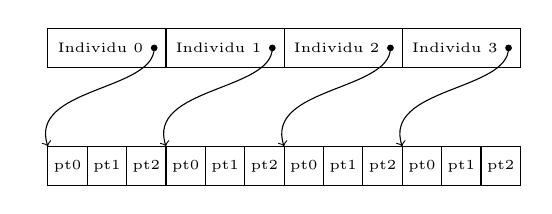
\begin{tikzpicture}
\foreach \x in {0,1,2,3}{
    \draw (1.5*\x,5) rectangle node {\tiny Individu \x~~~} (1.5*\x+1.5,4.5);
    
	\draw[->] (1.5*\x+1.35,4.75) .. controls (1.5*\x+1.35,4.2) and (1.5*\x-0.25,4.25) .. (1.5*\x,3.5);
	\draw[fill=black] (1.5*\x+1.35,4.75) circle (1pt);
	\foreach \y in {0,1,2}
    	\draw (1.5*\x+0.5*\y,3) rectangle node {\tiny pt\y} (1.5*\x+0.5*\y+0.5,3.5);
}

\end{tikzpicture}
\caption{De individu array en de punten array op de heap}
\end{figure}
Om de individuen bij te houden hebben we er voor gekozen ze in 1 lange rij op de heap te plaatsen. Dit zorgt ervoor dat we de populatiegrootte at runtime kunnen bepalen, wat handig kan zijn bij de parallelle  uitvoering. We houden ook 1 lange array van punten bij op de heap. Deze array bevat $n\cdot N_p$ punten. Elk van de individuen heeft een pointer die naar een plaats in deze array wijst. Het in één keer alloceren zorgt ervoor dat we tijdens de uitvoering geen overhead hebben door allocaties. Het zorgt er ook voor dat we minder gemakkelijk memory leaks enzo hebben.

\subsection{Plaats kideren}
Na het paren zijn er meer individuen in de populatie. Om deze een plaats in het geheugen te geven maken tijdens de initialisatie de arrays waarin we het in Sectie~\ref{sub:heap} hadden extra ``lege'' plaatsen. De kinderen worden dan gestokeerd vanaf index $N_p$.

Door deze grotere array te nemen wordt het ook gemakelijker om tournament selection to te passen op heel de populatie.

\subsection{Tests}
\label{sub:explain_tests}
Om te testen of bepaalde stukken code wel werkten hebben we testen geschreven. Deze zijn te vinden in \texttt{main.c} en kunnen worden geactiveerd met de \texttt{-D} vlag van de compiler.

\subsection{Debuging}
\label{sub:explain_debug_analyse}
Tijdens de ontwikkeling wilden we graag zien hoe de fitheid verliep in de tijd. Hiervoor hebben we een \texttt{log\_dbg} macro geintroduceerd die enkel print als er gecompileerd werdt met \texttt{-DDEBUG}.

Om de performantie gemakkelijk te testen met Python hebben we een {\em{Performance Print}} mode toegevoegd. Deze wordt geactiveerd door te compilen met  \texttt{-DPERFORMANCE\_PRINT}. In deze mode wordt enkel het aantal iteraties en de bekomen fitheid geprint.

% subsection  (end)
% section explainationcode (end)

%\section{Bronnen}
Er moet vermeld worden dat het \texttt{icosagon.poly} bestand afkomstig is van Jonathan Peck. We hebben dit bestand uitgewisseld om een andere figuur dan het gegeven vierkant te hebben samen met een notie van de maximale fitheid voor 50 punten in deze figuur. Code is er natuurlijk niet uitgewisseld.

\begin{thebibliography}{9}

\bibitem{lamport94}
  Haupt, Randy L., and Sue Ellen Haupt. ``Practical genetic algorithms.'' (2004).

\bibitem{baker85}
Baker, James Edward. "Adaptive selection methods for genetic algorithms." Proceedings of an International Conference on Genetic Algorithms and their applications. 1985.

\bibitem{parra9748125}
Pit, Laurens Jan. "Parallel genetic algorithms." MS (Computer Sci.) Dissertation (1995).

\bibitem{cuofiezafm}
Brinkmann, Gunnar. "Datastructuren en Algoritmen III, 2014." Cursus (2014)

\bibitem{MPIDOC}
University of Tennessee, "MPI: A Message-Passing Interface Standard" Online PDF. http://www.mpi-forum.org/docs/mpi-3.0/mpi30-report.pdf (2012)



\end{thebibliography}
\end{document}


\part{Parralelisering}
Nog niet gedaan...

\part{Beschouwing en conclusies}

\section{Bronnen}
Er moet vermeld worden dat het \texttt{icosagon.poly} bestand afkomstig is van Jonathan Peck. We hebben dit bestand uitgewisseld om een andere figuur dan het gegeven vierkant te hebben samen met een notie van de maximale fitheid voor 50 punten in deze figuur. Code is er natuurlijk niet uitgewisseld.

\begin{thebibliography}{9}

\bibitem{lamport94}
  Haupt, Randy L., and Sue Ellen Haupt. ``Practical genetic algorithms.'' (2004).

\bibitem{baker85}
Baker, James Edward. "Adaptive selection methods for genetic algorithms." Proceedings of an International Conference on Genetic Algorithms and their applications. 1985.

\bibitem{parra9748125}
Pit, Laurens Jan. "Parallel genetic algorithms." MS (Computer Sci.) Dissertation (1995).

\bibitem{cuofiezafm}
Brinkmann, Gunnar. "Datastructuren en Algoritmen III, 2014." Cursus (2014)

\bibitem{MPIDOC}
University of Tennessee, "MPI: A Message-Passing Interface Standard" Online PDF. http://www.mpi-forum.org/docs/mpi-3.0/mpi30-report.pdf (2012)



\end{thebibliography}
\end{document}
